\section{Le chiffrement asymétrique}
Inventé en 1977 par Diffie et Hellman
\cite{NewDirectionsInCryptography}, le chiffrement asymétrique, aussi
connu sous le nom de chiffrement à clé publique permet de résoudre le
problème de communication des clés du chiffrement symétrique, et
permet aussi l'authentification, en s'aidant des fonctions de hachage 
(chapitre \ref{sec:FonctionHachage}). 

Chaque utilisateur possède alors deux clés : une clé publique qu'il
distribue à tout le monde ainsi qu'une clé privée, qu'il garde
secrète. La clé publique permettra de chiffrer un message, que
l'utilisateur pourra déchiffrer grâce à sa clé privée. Ainsi,
seule la
personne en possession de la clé de déchiffrement (privée), le
destinataire donc, pourra déchiffrer le message. \\

Tout chiffrement à clé publique doit répondre aux quatre points
suivants, pour un algorithme de chiffrement $E$, un algorithme de
déchiffrement $D$, une clé quelconque $k$, un message clair $M$ et un
message chiffré $C$ : 
\begin{enumerate}
  \item $E$ est l'inverse de $D$, donc
    \begin{center}
      $D(E(M)) = M$
    \end{center}
  \item $E$ et $D$ sont faciles à calculer
  \item $D$ est introuvable si l'on connait $E$
  \item Si on applique l'opération de déchiffrement suivie de
    l'opération de chiffrement sur un message, on retrouve le message
    d'origine, ainsi
    \begin{center}
      $E(D(M)) = M$
    \end{center}
\end{enumerate}

C'est en fait l'opération de chiffrement qui est publique ou secrète
($E$ est publique, $D$ secrète), mais d'après le principe de
Kerckhoffs, le secret d'une opération de chiffrement doit être sa clé
et non la méthode en soi, il y aura donc une clé privée qui
influencera le comportement de $D$, et une clé publique qui
influencera le comportement de $E$. La fonction $E$ est appelée une
\emph{fonction à sens unique à brèche secrète} 
car elle est facilement calculable dans un sens, et extrêmement
compliquée à calculer dans l'autre,
%(elle est dite à \emph{sens unique})
sauf en connaissant la \emph{brèche} (la clé).

Pour ce qui est de la troisième proposition, on pourrait trouver $D$
via une recherche exhaustive (en essayant tous les cas possibles), ou
en essayant d'exploiter les liens liant $E$ à $D$ ; mais ce type
de recherche est impossible en pratique, à cause du nombre de
possibilités et des restrictions matérielles de calculs. Nous
expliquerons ceci plus en détail dans le chapitre
\ref{chap:Cryptanalyse} sur la cryptanalyse.

On peut donc considérer l'opération de chiffrement comme si on
mettait le message dans une boite, que l'on ferme avec un cadenas
dont seul le destinataire du message possède la clé.

\begin{figure}[h]
  \begin{center}
    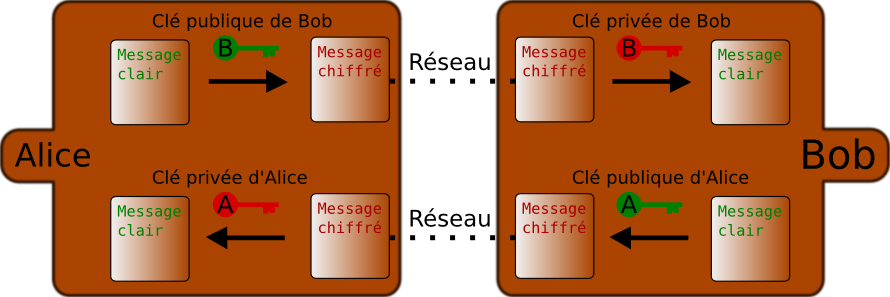
\includegraphics[scale=0.5]{images/ChiffrementAsymetrique.png}
  \end{center}
  \caption{le fonctionnement du chiffrement asymétrique, pour deux
    échanges de messages entre Alice et Bob.}
  \label{fig:ChiffrementSymetrique}
\end{figure}

Nous expliquerons les mécanismes d'authentification dans le 
chapitre \ref{sec:Authentification}. \\

\paragraph{Exemple : RSA}
Dans leur publication, Diffie et Hellman n'ont pas pu donner
d'exemple de système de chiffrement à clé publique. Le premier
système de ce genre est mis au point en 1977 par Adi Shamir, Rom
Rivest et Len Adleman, et publié en 1978 \cite{RSAPaper}.
La force de cette méthode réside dans la difficulté à factoriser
un nombre qui est le produit de deux très grands nombres premiers. 

RSA se base donc sur le choix de deux nombres premiers, que nous
nommerons $p$ et $q$.
La clé publique est le couple $(e,n)$ tel que $n = p q$ et $e$ est
premier\footnote{Deux nombres sont entiers
entre eux si et seulement si leur plus grand commun diviseur est 1.}avec $(p-1) (q-1)$.
Pour l'encodage, on convertit d'abord notre message en une suite
d'entiers $M_1, M_2, \dots, M_n$, % TODO parler de l'ascii ?
que nous coderons ainsi :
\begin{center}
  $C_i = (M_i)^e ~mod~n$
\end{center}

La clé privée est formée par le couple $(d,n)$, tel que
$e d = 1 [mod (p-1) (q-1)]$.
Pour déchiffrer le message chiffré composée des entiers $C_1. C_2,
\dots, C_n$, on applique la formule
\begin{center}
  $M_i = (C_i)^d ~mod~n$
\end{center}


